\documentclass[12pt,twosides,onecolumn,openany]{article}
\usepackage{graphicx} 

\usepackage{cite}
\usepackage[catalan]{babel}
\usepackage{emptypage}
\usepackage{hyperref}
\usepackage{mathtools}
\usepackage{blindtext}
\usepackage[utf8]{inputenc}
\usepackage{caption}
\usepackage{subcaption}
\usepackage{wrapfig}
\usepackage[a4paper]{geometry}
\geometry{top=2.5cm, bottom=2.5cm, left=2.5cm, right=2.5cm}
\usepackage{fancyhdr}
\pagestyle{fancy}
\usepackage{amsmath}
\usepackage{amssymb}
\usepackage{amsfonts}
\providecommand{\norm}[1]{\lVert#1\rVert}
\hypersetup{colorlinks=true,urlcolor=blue,linkcolor=blue}
\usepackage{multirow}
\usepackage{multicol}
\usepackage{rotating}

\usepackage{titlesec}

\newenvironment{Figura}
  {\par\medskip\noindent\minipage{\linewidth}}
  {\endminipage\par\medskip}

\titleformat{\section}  % comando de sección a formatear
  {\fontsize{14}{16}\bfseries} % formato para toda la línea
  {\thesection} % cómo mostrar el número
  {0.4em} % espacio entre el número y el texto
  {} % formato solo para el texto
  [] % formato para después del texto


\fancyhf{}
\fancyhead[LO,RE]{Grup D3}
\fancyhead[RO,LE]{Pràctica IVc}
\fancyfoot[LO,RE]{\thepage}
\fancyfoot[RO,LE]{Laboratori de Termodinàmica - UAB}
\graphicspath{ {images/} }

\begin{document}

\begin{center}
    {\Large \textsc{Transicions de fase: Tècniques de buit i Punt triple d’un sistema}}\\
    \vspace{0.2cm}
    \textsc{28 d'Octubre de 2024}\\
    \vspace{0.2cm}
    $\begin{matrix} 
    \text{Miguel A.} \hspace{1.5cm} & \text{Daniel B.} & \hspace{1.5cm} \text{Sergi R.}\\1637738 \hspace{1.5cm} & 1603508 & \hspace{1.5cm} 1607805
    \end{matrix}$
\end{center}
\begin{center}
    \textsc{\textit{RESUM}}
\end{center}
Aquesta pràctica de laboratori se centra en la determinació de la pressió límit de buit de dos sistemes diferents d'obtenció de buit, la trompa d'aigua i la bomba d'oli rotativa a paletes. Es realitza una comparació entre els dos sistemes i, amb la més adient (bomba d'oli) es realitzen mesures per a obtenir les coordenades de punt triple del ciclohexà.
\vspace{0.5cm}
\begin{multicols}{2}
\section{Introducció i objecctius}
A l'hora de fer servir com a aparell de mesura de la pressió un manòmetre de mercuri és necessari considerar alguna correcció. Un manòmetre de mercuri està format per un tub en forma de "u", amb un extrem connectat obert a l'atmosfera i l'altre connectat al sistema el qual volem mesurar-ne la pressió. Aquest aparell aprofita la incompressibilitat del mercuri per a obtenir mesures de pressió a partir de les mesures de l'alçada relativa entre la primera meitat del tub (corresponent a la oberta, mesurant una alçada $h_1$) i la segona meitat del tub (corresponent a la connectada al sistema, mesurant una alçada $h_2$). A partir d'aquesta diferència i tenint en compte que al laboratori també participa la pressió atmosfèrica $p_{\text{atm}}$ (que mesurem amb un baròmetre), podem calcular la pressió observada al laboratori del nostre sistema com 
\begin{equation}\label{p_obs}
    p_{\text{obs}} = p_{\text{atm}} + \Delta h
\end{equation}
on $\Delta h = h_1 - h_2$.\\\\
A aquestes mesures observades de pressió han de passar per una o més correccions. La primera i més important és la correcció de temperatura. Aquesta correcció considera l'error provocat per la dilatació del mercuri amb la temperatura. El manòmetre de mercuri està cal·librat a una determinada temperatura, \(0 \,^\circ\text{C}\). Per tant, obtenim les mesures de pressió del sistema calculant, a partir de lo obtingut a l'Equació \eqref{p_obs}
\begin{equation}\label{correcció_manomètrica}
    p_{\text{sist}} = \frac{p_{\text{obs}}}{1+\alpha(T_{\text{lab}} - T_{\text{cal}})}
\end{equation}
on $\alpha$ és el coeficient de dilatació del mercuri, amb un valor de \( \alpha = 8,3\cdot 10^{-4} \, \text{K}^{-1}\), $T_{\text{lab}}$ és la temperatura mesurada del laboratori i $T_{\text{cal}}$ és la temperatura a la que s'ha realitzat el calibratge del manòmetre.\\\\
Els objectius d'aquesta pràctica són, a la primera part, comparar el funcionament de dos aparells d'obtenció de buit diferents realitzant mesures amb un manòmetre de mercuri i, a la segona part, trobar amb el sistema de buit més adient les coordenades de punt crític d'una mostra de ciclohexà.\\\\
Els sistemes d'obtenció de buit que es fan servir són la trompa d'aigua i la bomba d'oli rotativa a paletes. El primer obté buit a partir de l'efecte Venturi, fent passar un cabal d'aigua per un conducte estret. El segón obté buit a partir de la captura d'aire del sistema a partir de rotors amb paletes. Per tal de que aquest sistema estigui lubricat i hagi fuites d'aire mínimes que tornin al nostre sistema s'omple d'oli. Tant l'aigua per a la trompa com l'oli per a la bomba, com veurem, caracteritzen la limitació d'obtenció de buit. Aquesta limitació correspón a la pressió de vapor de cada substància.
\section{Resultats i discussió}
\subsection{Tècniques de buit}
Per a poder aplicar la correcció de temperatura al manòmetre de mercuri primer de tot mesurem la temperatura del laboratori abans i desprès de realitzar les mesures de pressió. Fent la mitjana de les dues mesures obtenim que el laboratori es troba a
\begin{equation*}
    T_{\text{lab}} = (23,2\pm0,1)\, ^\circ\text{C}
\end{equation*}
Realitzant les mesures de pressió per a cada sistema de buit obtenim les dades que s'observen a la Taula \ref{tau:mesures_alçada}.
\renewcommand{\arraystretch}{1.6}
\begin{Figura}
    \centering
    \captionof{table}{\footnotesize{Datos de alturas del manoemtro y cosas derivadas}}
    \begin{tabular}{c|c|c}
        $p_{\text{obs}}$ $\backslash\backslash$ Fluid  & \multirow{1}{1.6cm}{\centering Aigua} & \multirow{1}{1.6cm}{\centering Oli} \\
        \hline\hline
        \(h_{1}\,(\pm 1) \, \text{mmHg}\) & 52 & 40 \\
        \(h_{2}\,(\pm 1) \, \text{mmHg}\) & 783 & 790 \\
        \hline
        \( \Delta h \, (\pm 1,4) \, \text{mmHg}\) & -731 & -750
    \end{tabular}
    \label{tau:mesures_alçada}
\end{Figura}
A partir de les dades obtingudes apliquem la correcció de temperatura aplicant l'Equació \eqref{correcció_manomètrica} i obtenim la pressio del sistema per a cada mètode de buit:
\begin{equation*}
    p_{\text{sist}}^{\text{(a)}} = (21,4\pm1,4)\, \text{mmHg}
\end{equation*}
per a la trompa d'aigua,
\begin{equation*}
    p_{\text{sist}}^{\text{(o)}} = (2,7\pm1,4)\, \text{mmHg}
\end{equation*}
per a la bomba d'oli.\\\\
Podem observar com clarament les pressions límits de buit de cada sistema són diferents. La bomba rotatoria d'oli ens fa obtenir un buit més alt que la trompa d'aigua. Com s'ha mencionat a la introducció, aquesta limitació prové de la pressió de vapor del fluid que participa en el procés de buit. Per a comprovar això podem comparar la pressió límit obtinguda amb la trompa amb la pressió de vapor de l'aigua al voltant de la temperatura del laboratori, aquesta dada està tabulada a la literatura. Si volguessim comprovar-ho també amb la bomba d'oli necessitariem més informació, tant un estudi de la qualitat de construcció de la bomba com quin oli es fa servir per a libricar les peces rotatories. El valor de la pressió de vapor de l'aigua a \(23\,^\circ\text{C}\) és \cite{llibre_lab}
\begin{equation*}
    p_{\text{H}_2\text{O}}^{\text{vap}}= 21,068 \,\text{mmHg}
\end{equation*}
Es veu que la mesura obtinguda, tot i aproximar-se molt, tenint en compte la incertesa no entra en aquest valor tabulat. Podem explicar aquesta discrepància amb que, per a obtenir dades correctes de pressió amb el manòmetre de mercuri encara s'han de realitzar dues correccions més. La correció de dilatació amb la temperatura és la més significativa, per això el valor ens dona ben aproximat, però seguidament es poden realitzar correccions de gravetat (depenents de la latitud a on realitzem l'experiment) i correccions de capilaritat (depenents del comportament del menisc del mercuri al manòmetre).\\\\
La correcció per gravetat es realitza en la mesura de la pressió baromètrica un cop s'ha realitzat la correcció de temperatura. El laboratori on s'ha realitzat la mesura\footnote{UAB Campus Universitari, Bellaterra, Catalunya} es troba a una latitud d'aproximadament \(40 \,^\circ\text{N}\). Per a aquesta latitud s'ha de corregir la mesura de $p_{\text{lab}}$ en \(-0,39 \, \text{mmHg}\) \textit{citar libro Suriñach}. Aplicant la correcció i tornant a fer els càlculs obtenim\footnote{Podem realitzar la mateixa correcció amb la mesura de la pressió límit amb la bomba d'oli. El valor obtingut és: \(\hat{p}_{\text{sist}}^{\text{(o)}} = (2,4\pm1,4) \, \text{mmHg}\)} 
\begin{equation*}
    \hat{p}_{\text{sist}}^{\text{(a)}} = (21,0\pm1,4) \, \text{mmHg}
\end{equation*}
Observem que la correcció fa que el valor teòric entri dins de la incertesa del nostre resultat experimental. Encara es podria fer una aproximació més, com s'ha mencionat, per capilaritat. Per a calcular aquest error és necessari tenir informació de la que no disposem en aquesta pràctica. És necessari saber, amb una precissió de l'ordre de les dècimes de mil·limetre, el diàmetre del tub que conforma el manòmetre.\\\\
Hem comprovat doncs que efectivament la pressió límit de sistemes de buit com la trompa d'aigua ve caracteritzada per la pressió de vapor de l'aigua. En cas de voler fer servir l'efecte Venturi per a fer el buit i conseguir pressions més baixes seria necessari utilitzar un fluid amb una pressió de vapor més baixa com en el cas de la bomba d'oli.\\\\
Buscant algunes opcions al mercat d'oli per a màquines de buit podem veure com l'estàndard garantitza una pressió de vapor molt menor a un mil·límetre de mercuri \cite{shell}\cite{feroca}. Podem notar en les nostres mesures que això no es compleix. Aquesta incoherència amb les dades que prenem de referència es pot explicar si tenim en compte que és possible que el sistema de buit de la nostra bomba d'oli no estigui funcionant en condicions òptimes. Existeix la possibilitat de que l'aire que ha d'absorbir l'oli es filtri a través de les juntes de les peces rotatòries. Això fa que obtinguem un buit de pitjor qualitat, i podria explicar els nostres resultats.
\subsection{Punt triple d'un sistema}
Fem servir el segon muntatge experimental i prenem dades de temperatura, pressió i temps per al camí realitzat per a arribar al punt triple. Per a poder escollir un sistema de buit adient primer hem de revisar les coordenades del punt triple del ciclohexà tabulades a la literatura. Aquestes coordenades \cite{punt_triple} corresponen als valors de
\begin{equation*}
    \bar{T}_{\text{triple}} = 6,32 \, ^\circ\text{C}
\end{equation*}
i de
\begin{equation*}
    \bar{p}_{\text{triple}} = 40,41 \, \text{mmHg}
\end{equation*}
Segons aquestes dades podem considerar més adient fer servir la bomba d'oli i no la trompa d'aigua per a trobar el punt triple del ciclohexà, ja que és un sistema que deixa més marge entre el seu límit i la mesura que estem buscant de pressió.\\\\
S'observa a la Figura \ref{fig:completa} les repressentacions de les dades obtingudes, és a dir, de les evolucions temporals de $p$ i $T$ i del diagrama de fases $p$ vs $T$.
\end{multicols}
\begin{figure}[h]
    \centering
    \begin{subfigure}[b]{0.328\textwidth}
        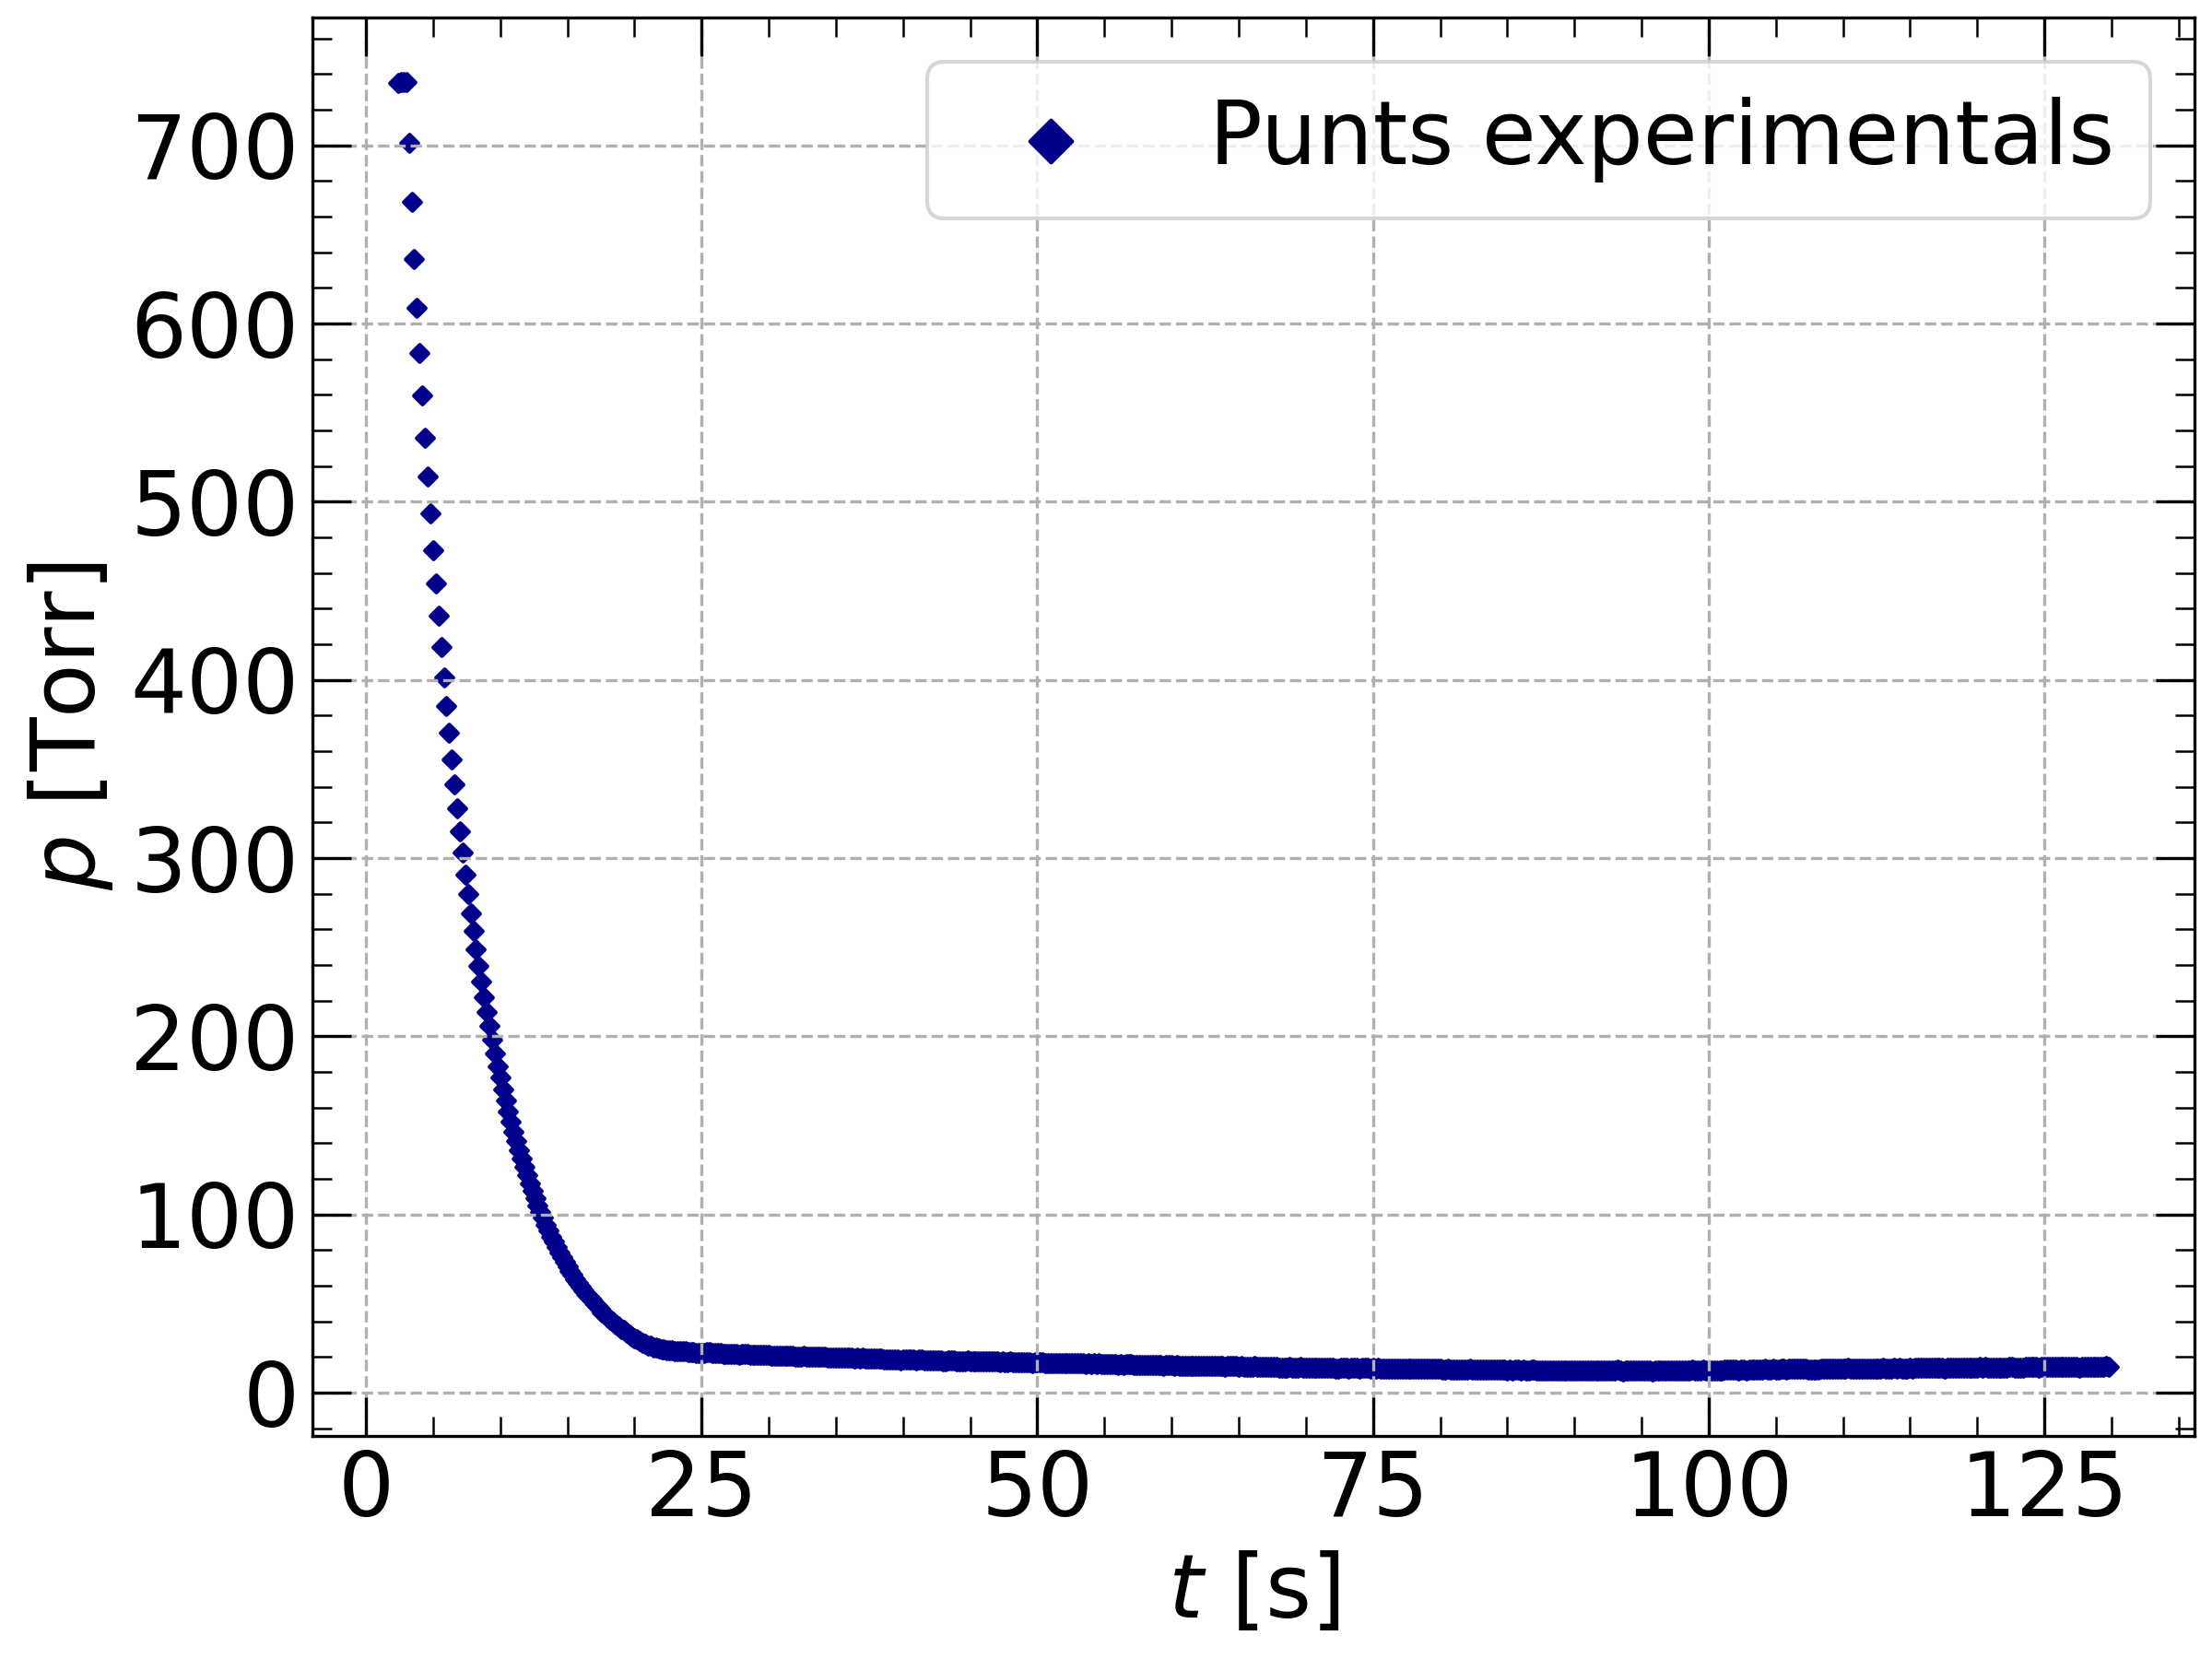
\includegraphics[width=\textwidth]{../../graphs/practica_IVc/plots/p_vs_t.png} 
        \caption{}
        \label{fig:p_vs_t_sencer}
    \end{subfigure}
    \hfill
    \begin{subfigure}[b]{0.328\textwidth}
        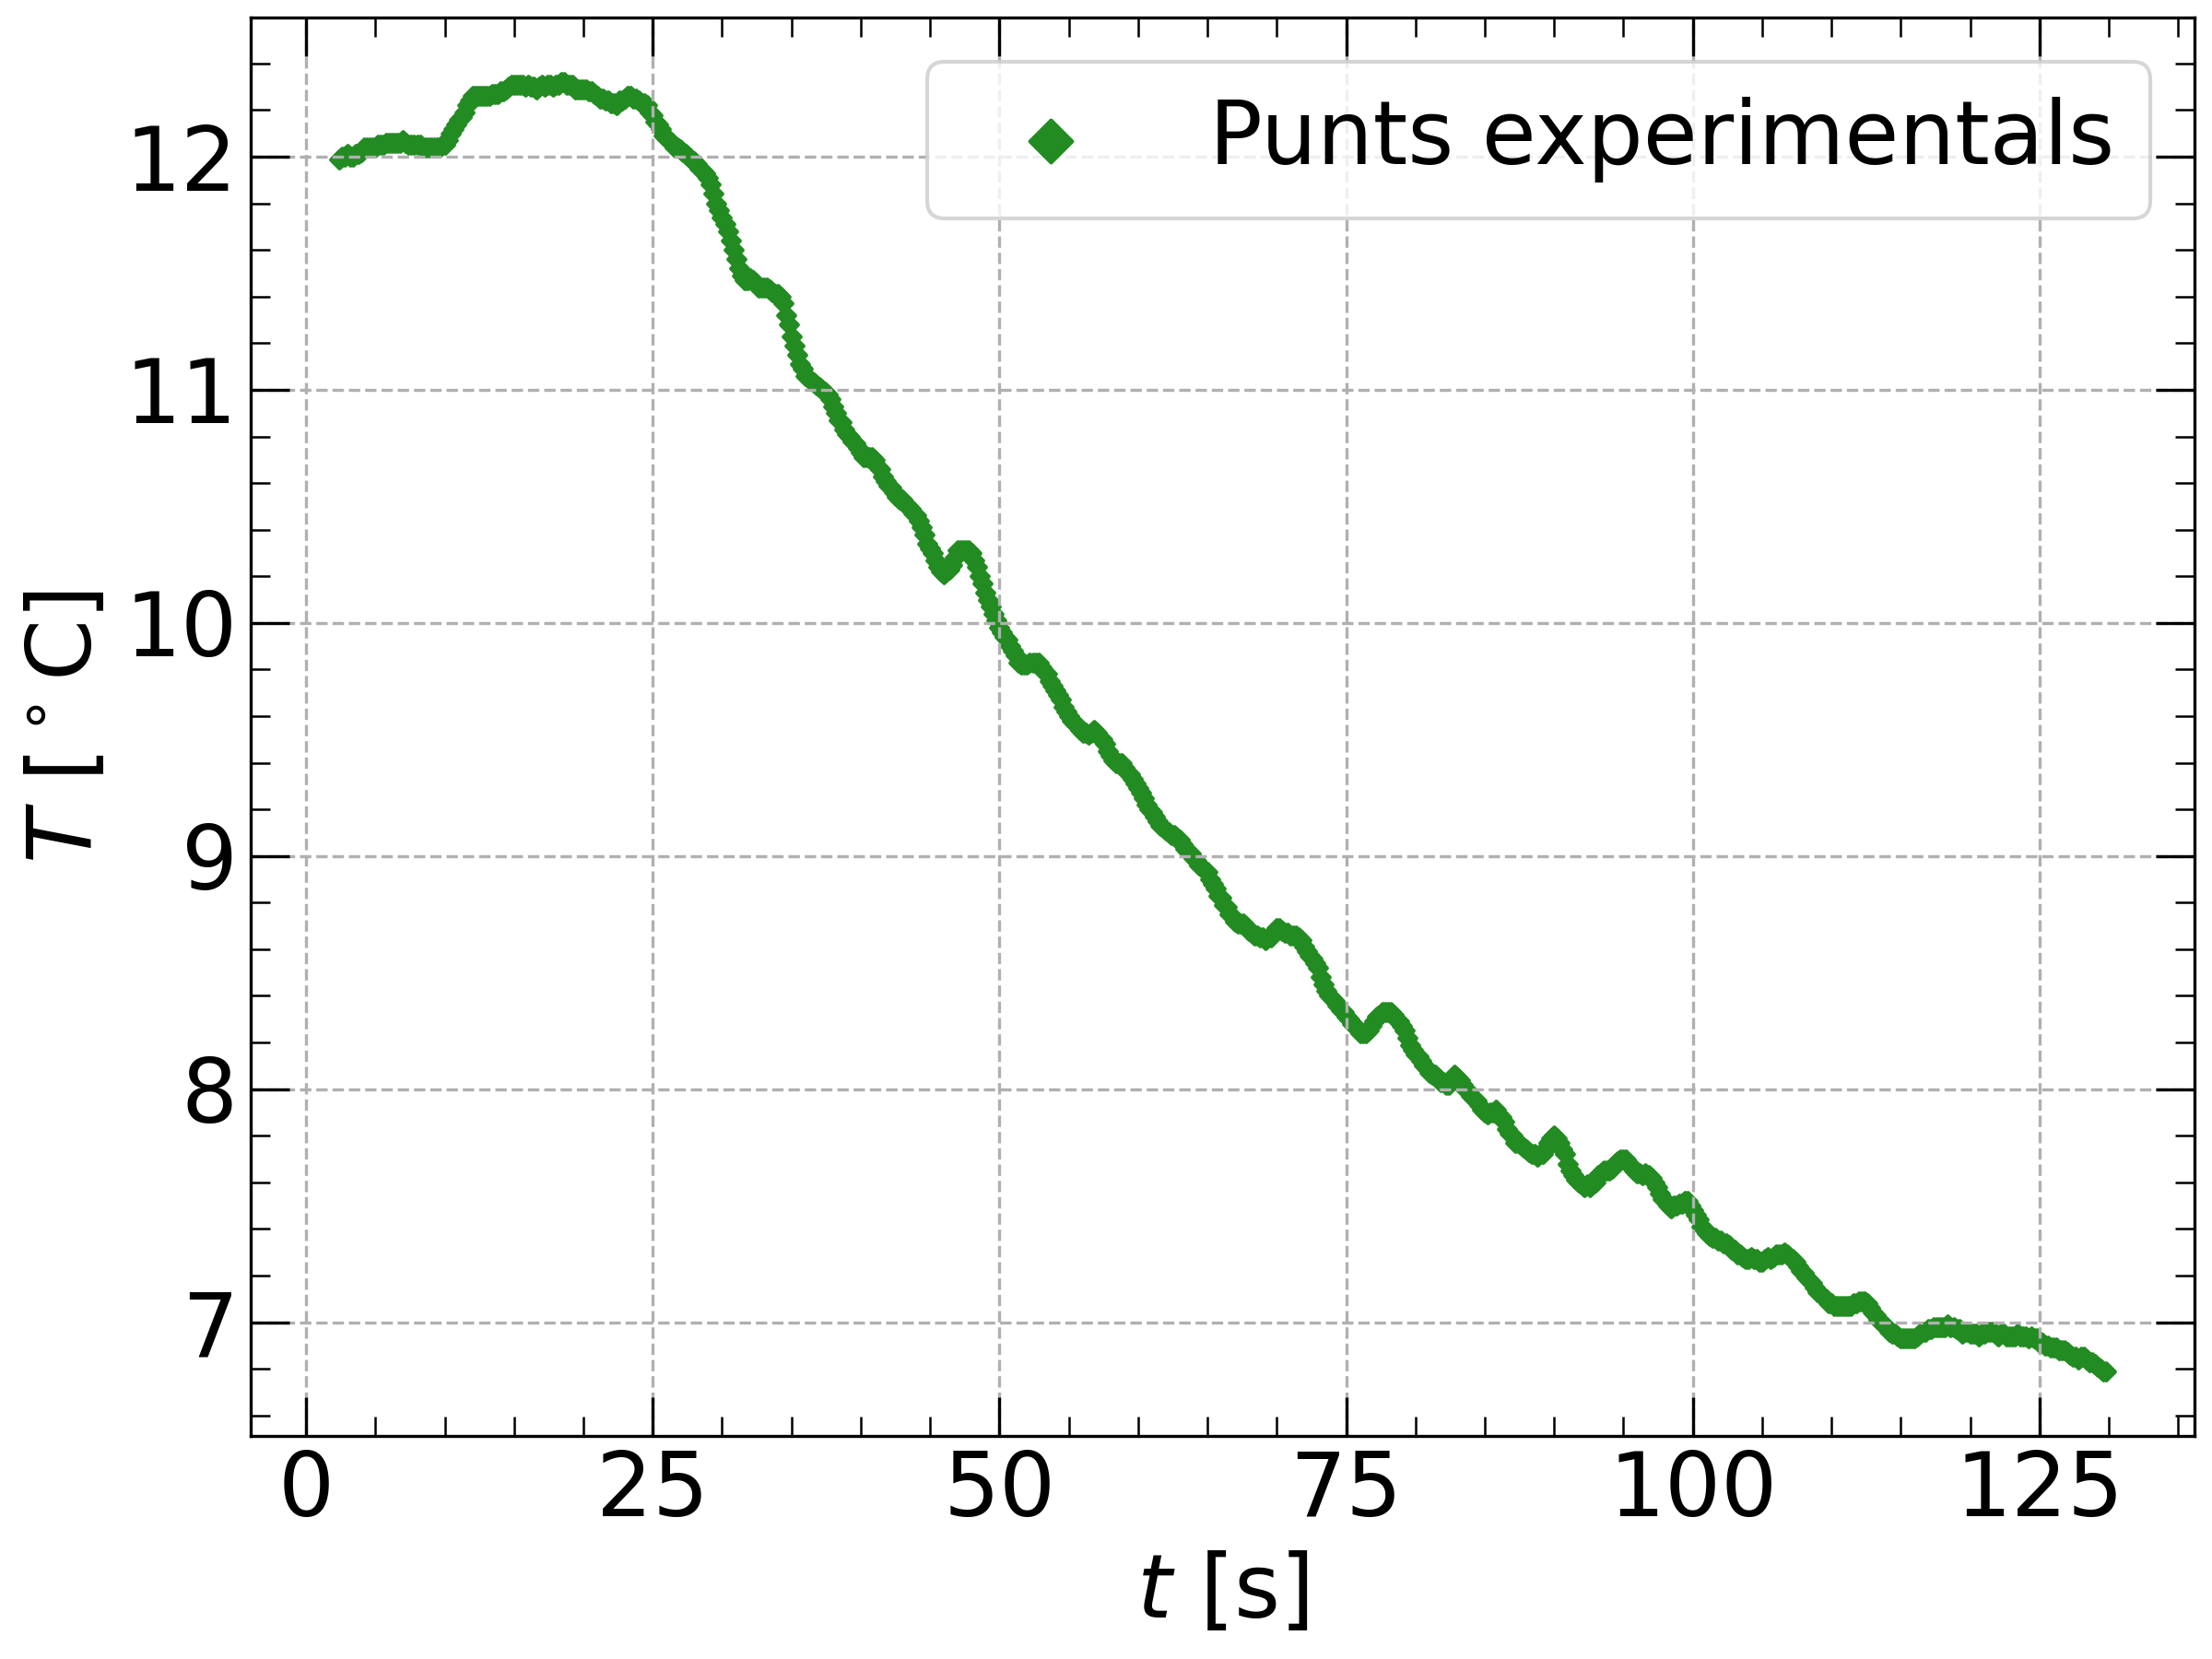
\includegraphics[width=\textwidth]{../../graphs/practica_IVc/plots/T_vs_t.png}
        \caption{} 
        \label{fig:T_vs_t_sencer}
    \end{subfigure}
    \hfill
    \begin{subfigure}[b]{0.328\textwidth}
        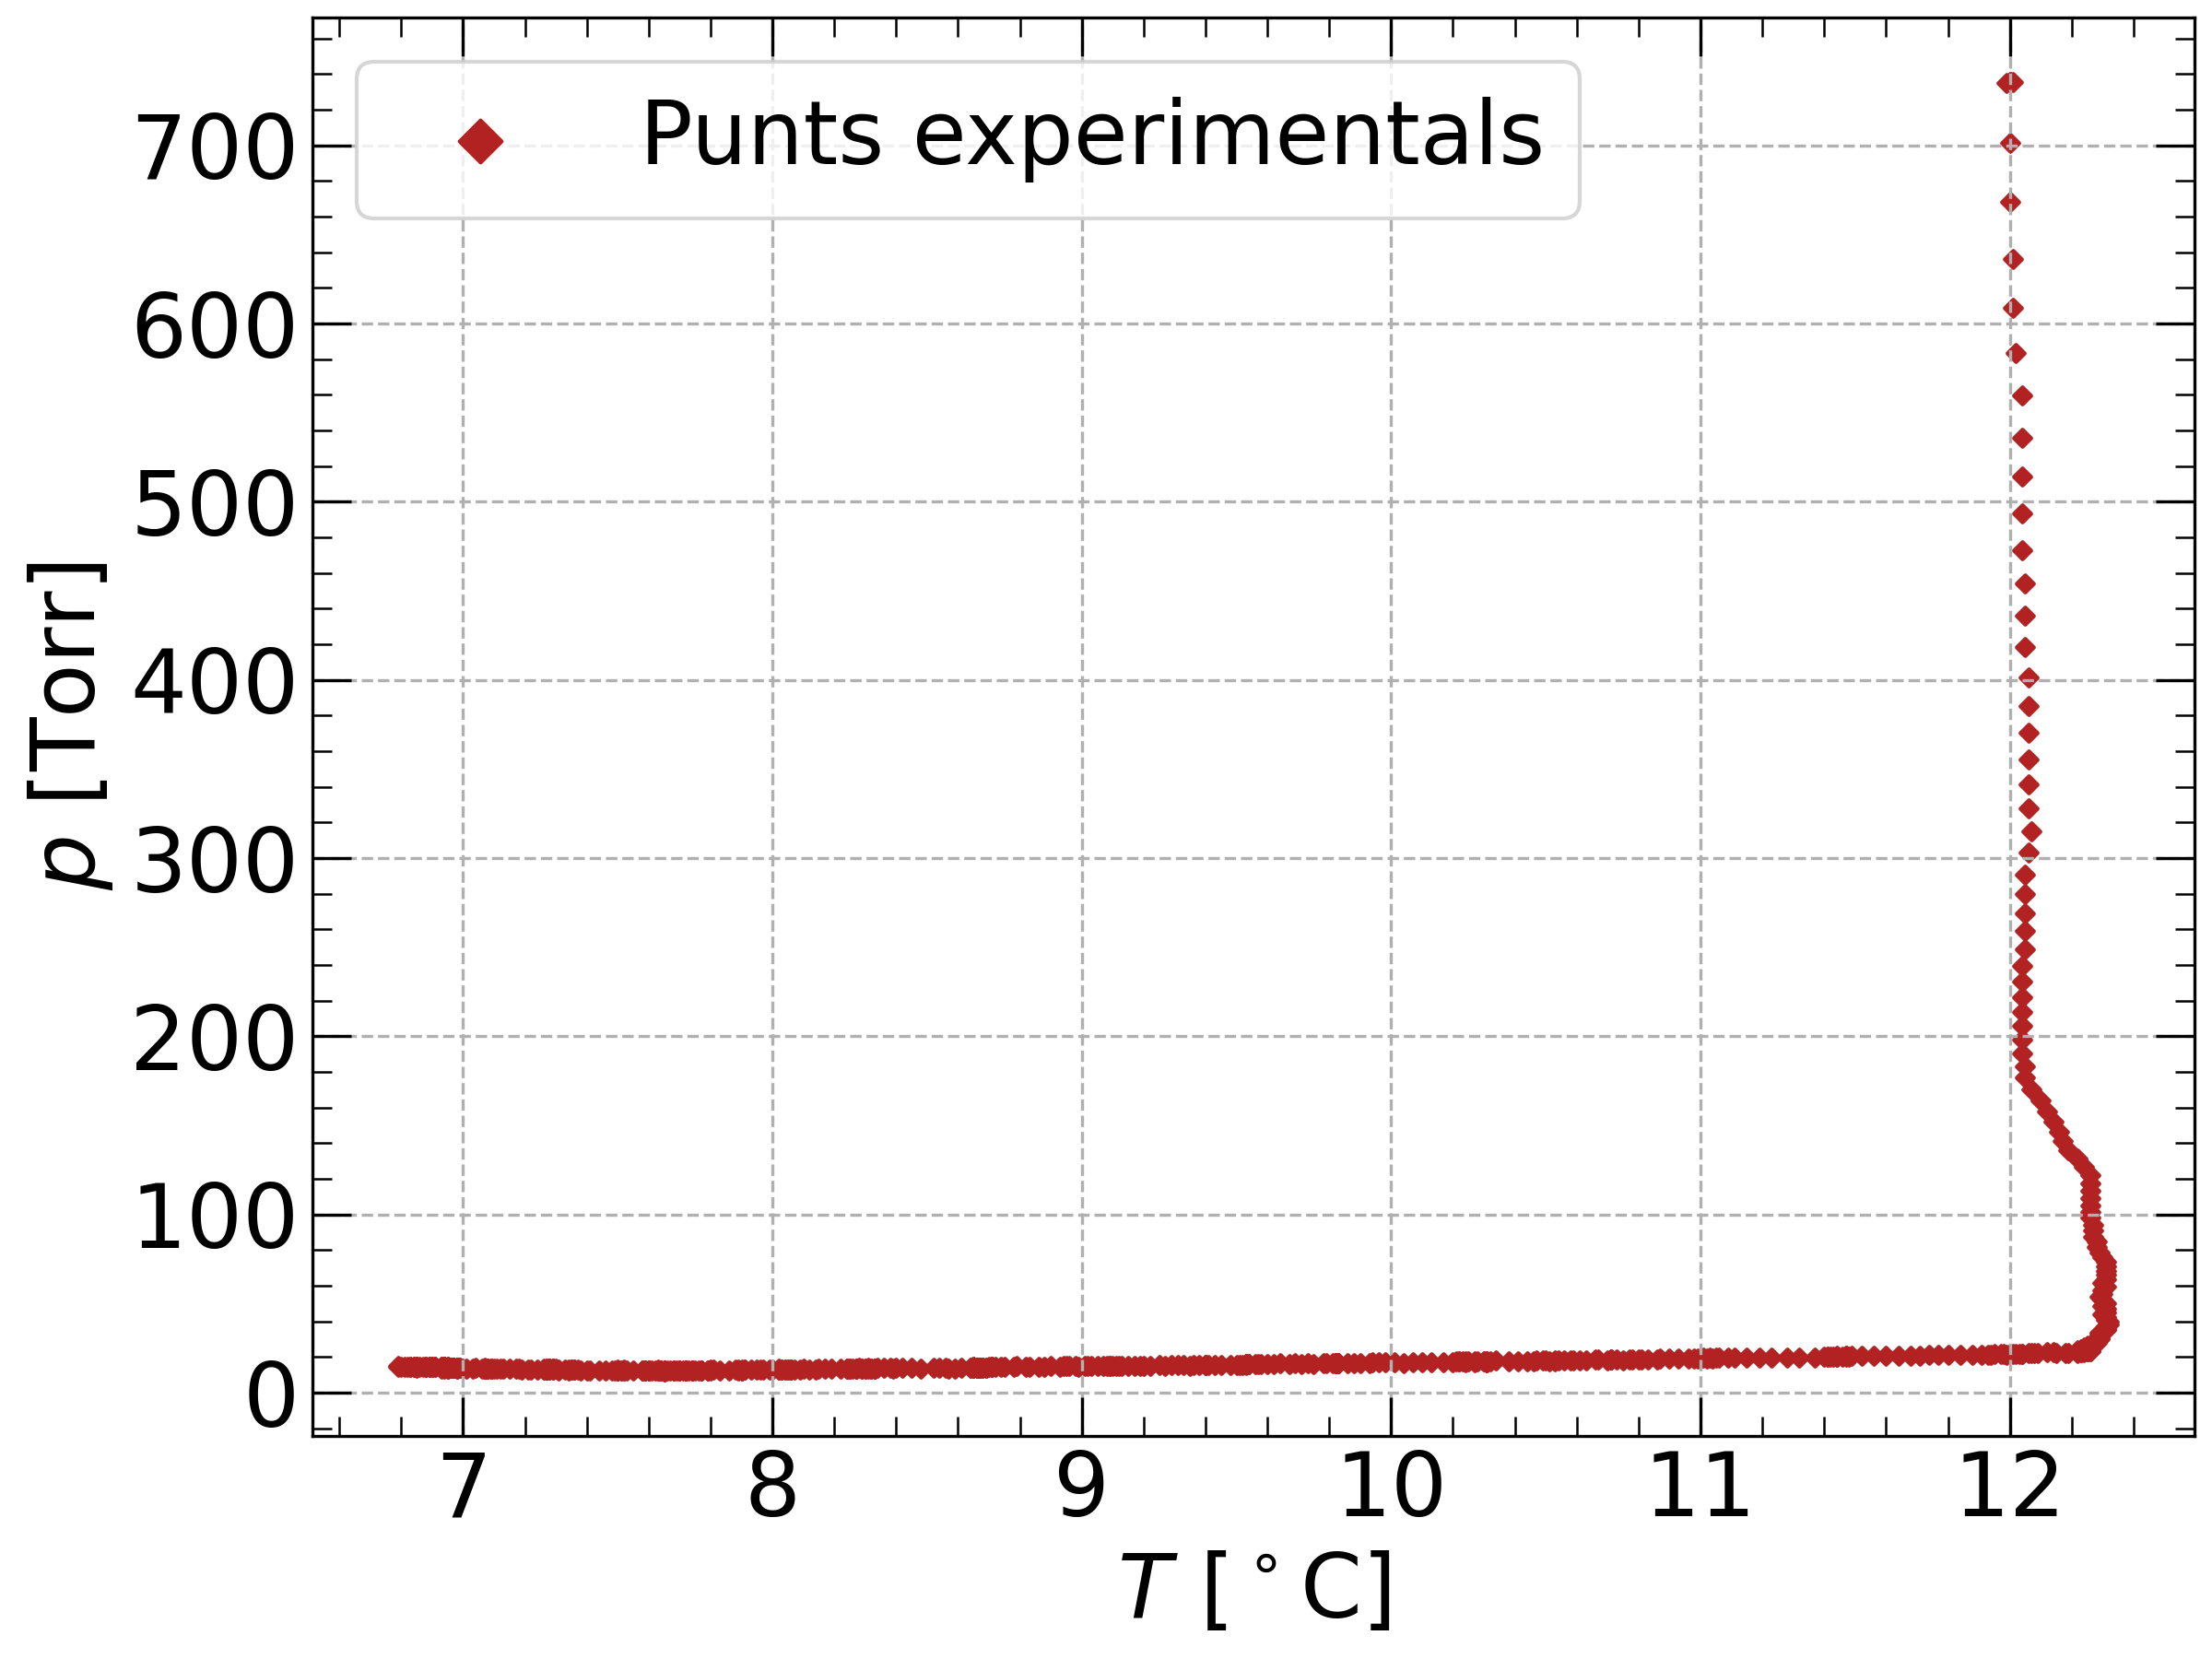
\includegraphics[width=\textwidth]{../../graphs/practica_IVc/plots/diagrama_de_fases.png}
        \caption{} 
        \label{fig:p_vs_T_sencer}
    \end{subfigure}
    \caption{(a) {\footnotesize Mesures experimentals d'evolució temporal completa de $p$.} (b) {\footnotesize Mesures experimentals d'evolució temporal completa de $T$. S'observa com la temperatura pren valors de forma oscil·lant.} (c) {\footnotesize Diagrama de fases $p$ vs $T$ complet del ciclohexà obtingut experimentalment. Es poden distingir els dos camins recorreguts per arribar al punt triple, un primer baixant la pressió de forma aproximadament isotèrmica, l'altre baixant per la corva d'equilibri vapor-líquid del ciclohexà. Al ser molt petites, s'ometen les incerteses a les tres repressentacions.}}
    \label{fig:completa}
\end{figure}
\newpage
\begin{figure}[h]
    \centering
    \begin{subfigure}[b]{0.328\textwidth}
        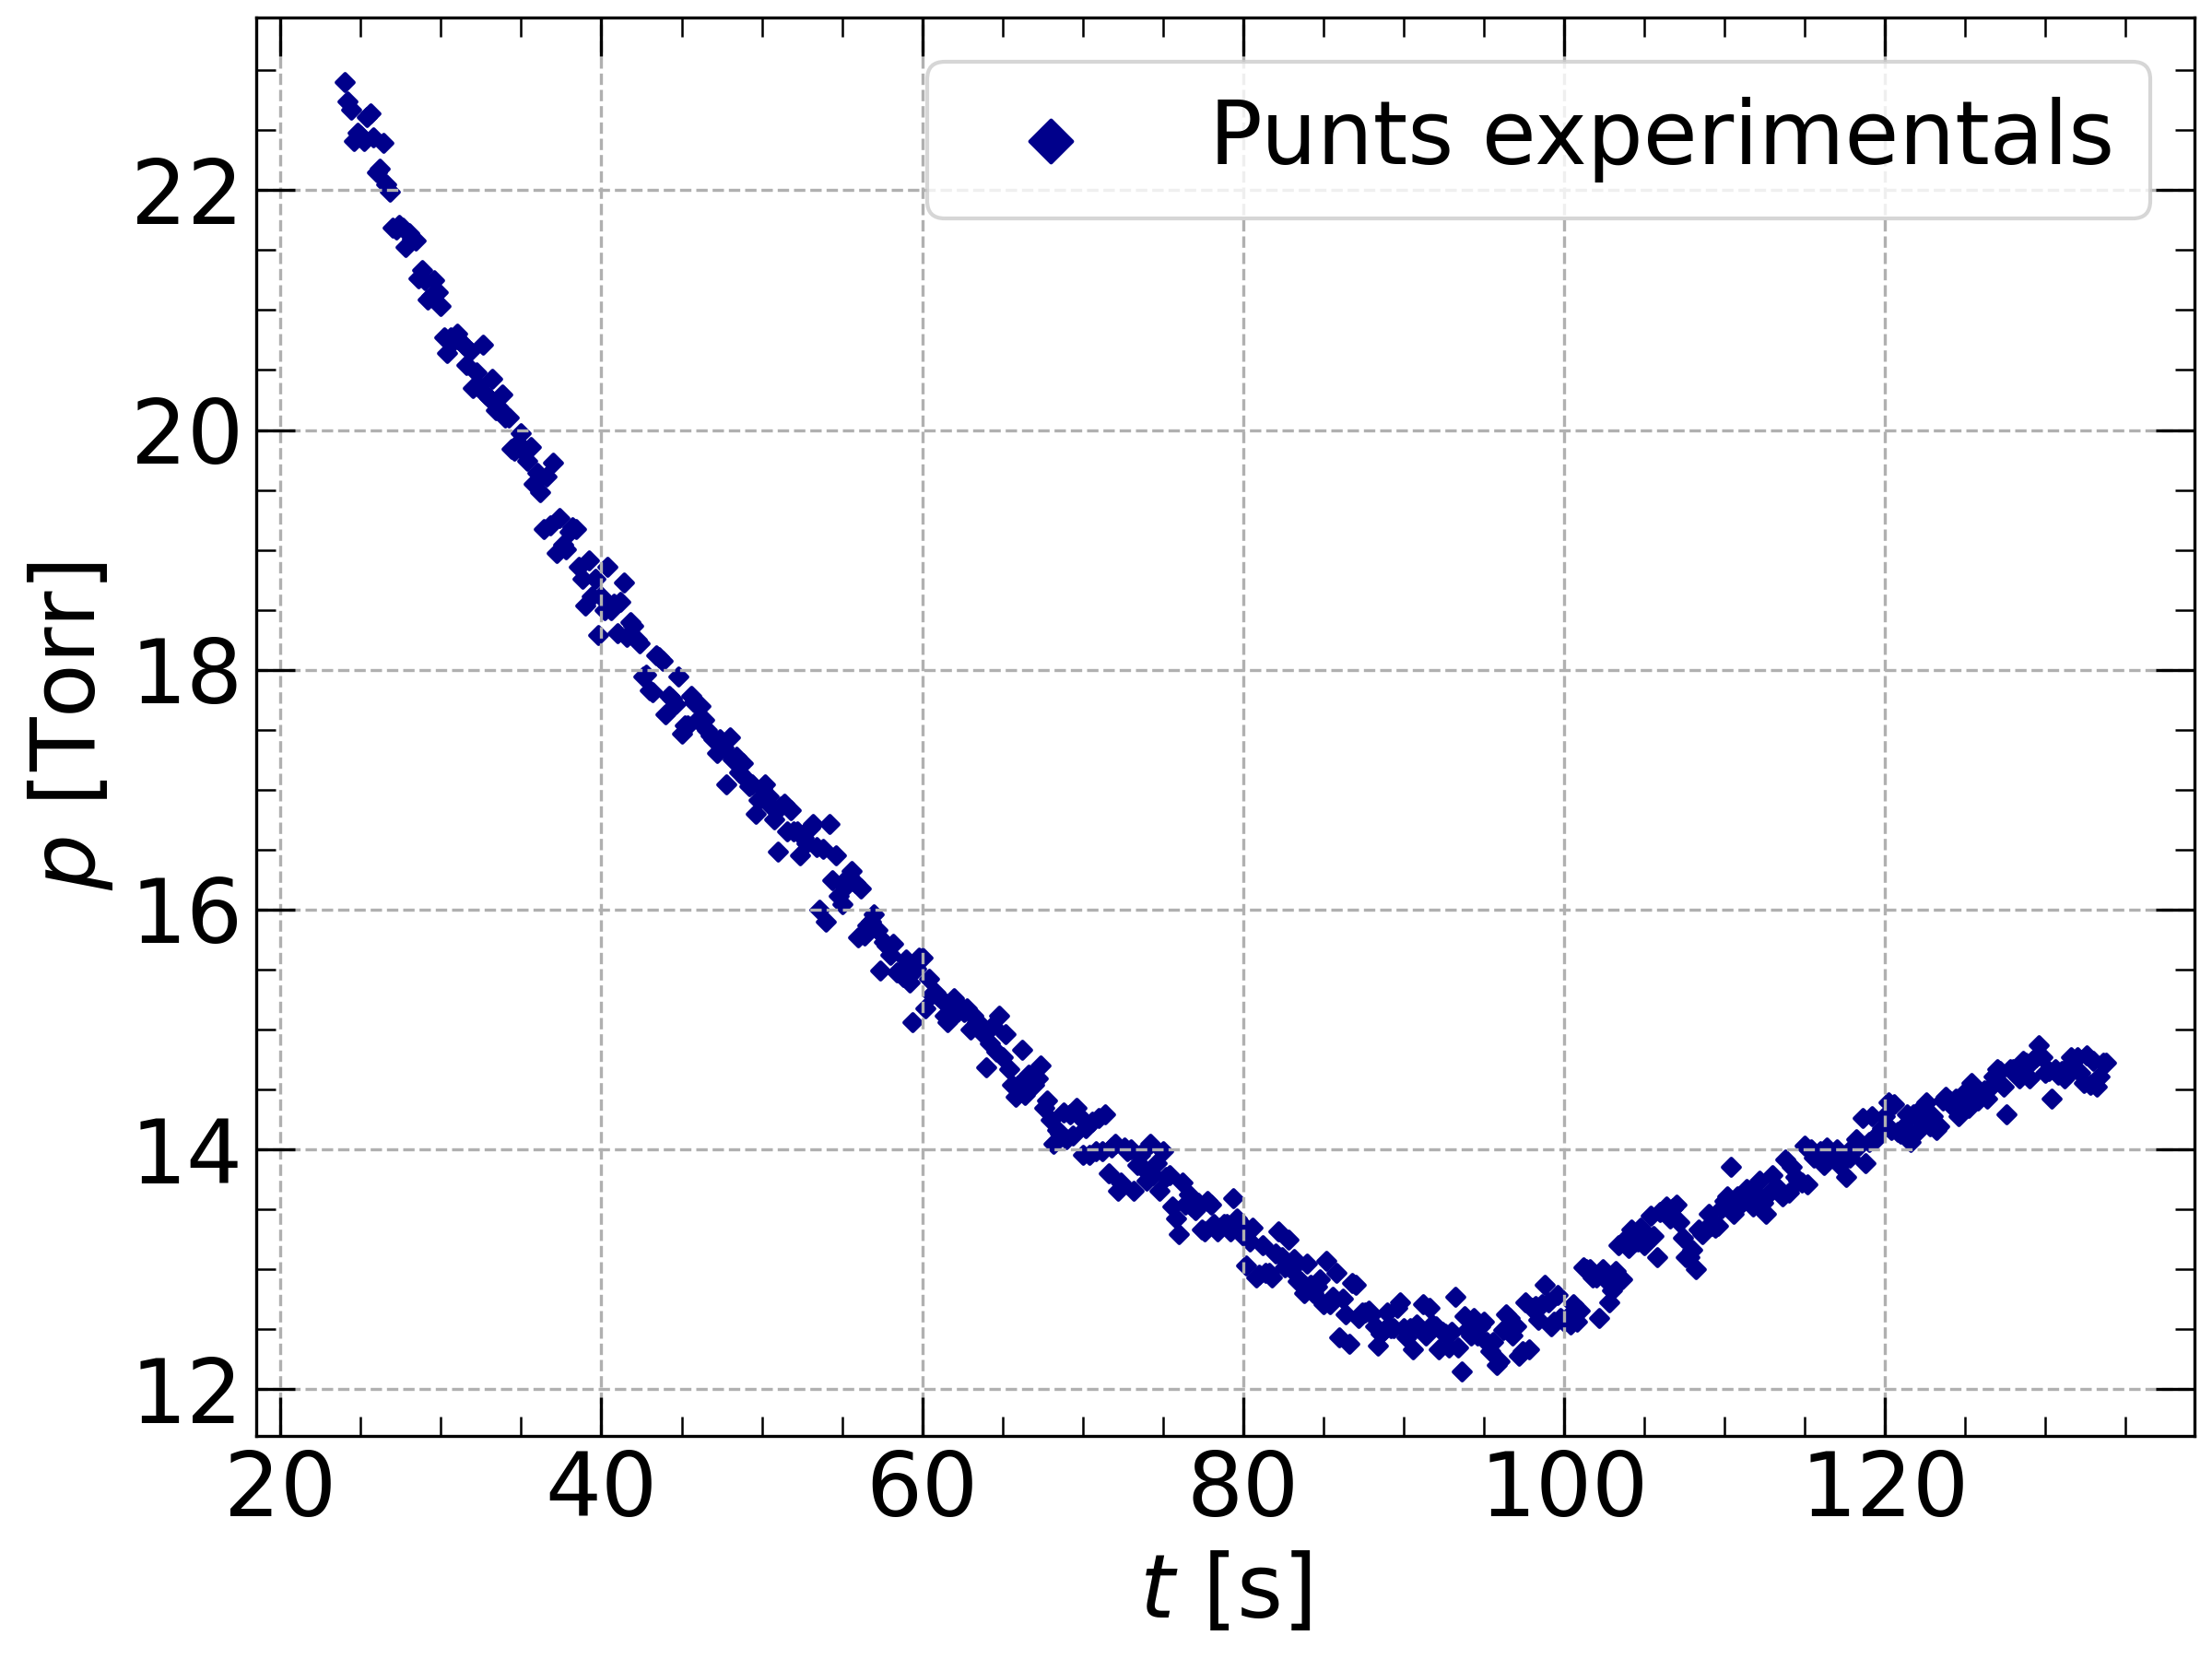
\includegraphics[width=\textwidth]{../../graphs/practica_IVc/plots/p_vs_t_tallat.png} 
        \caption{}
        \label{fig:p_vs_t_tallat}
    \end{subfigure}
    \hfill
    \begin{subfigure}[b]{0.328\textwidth}
        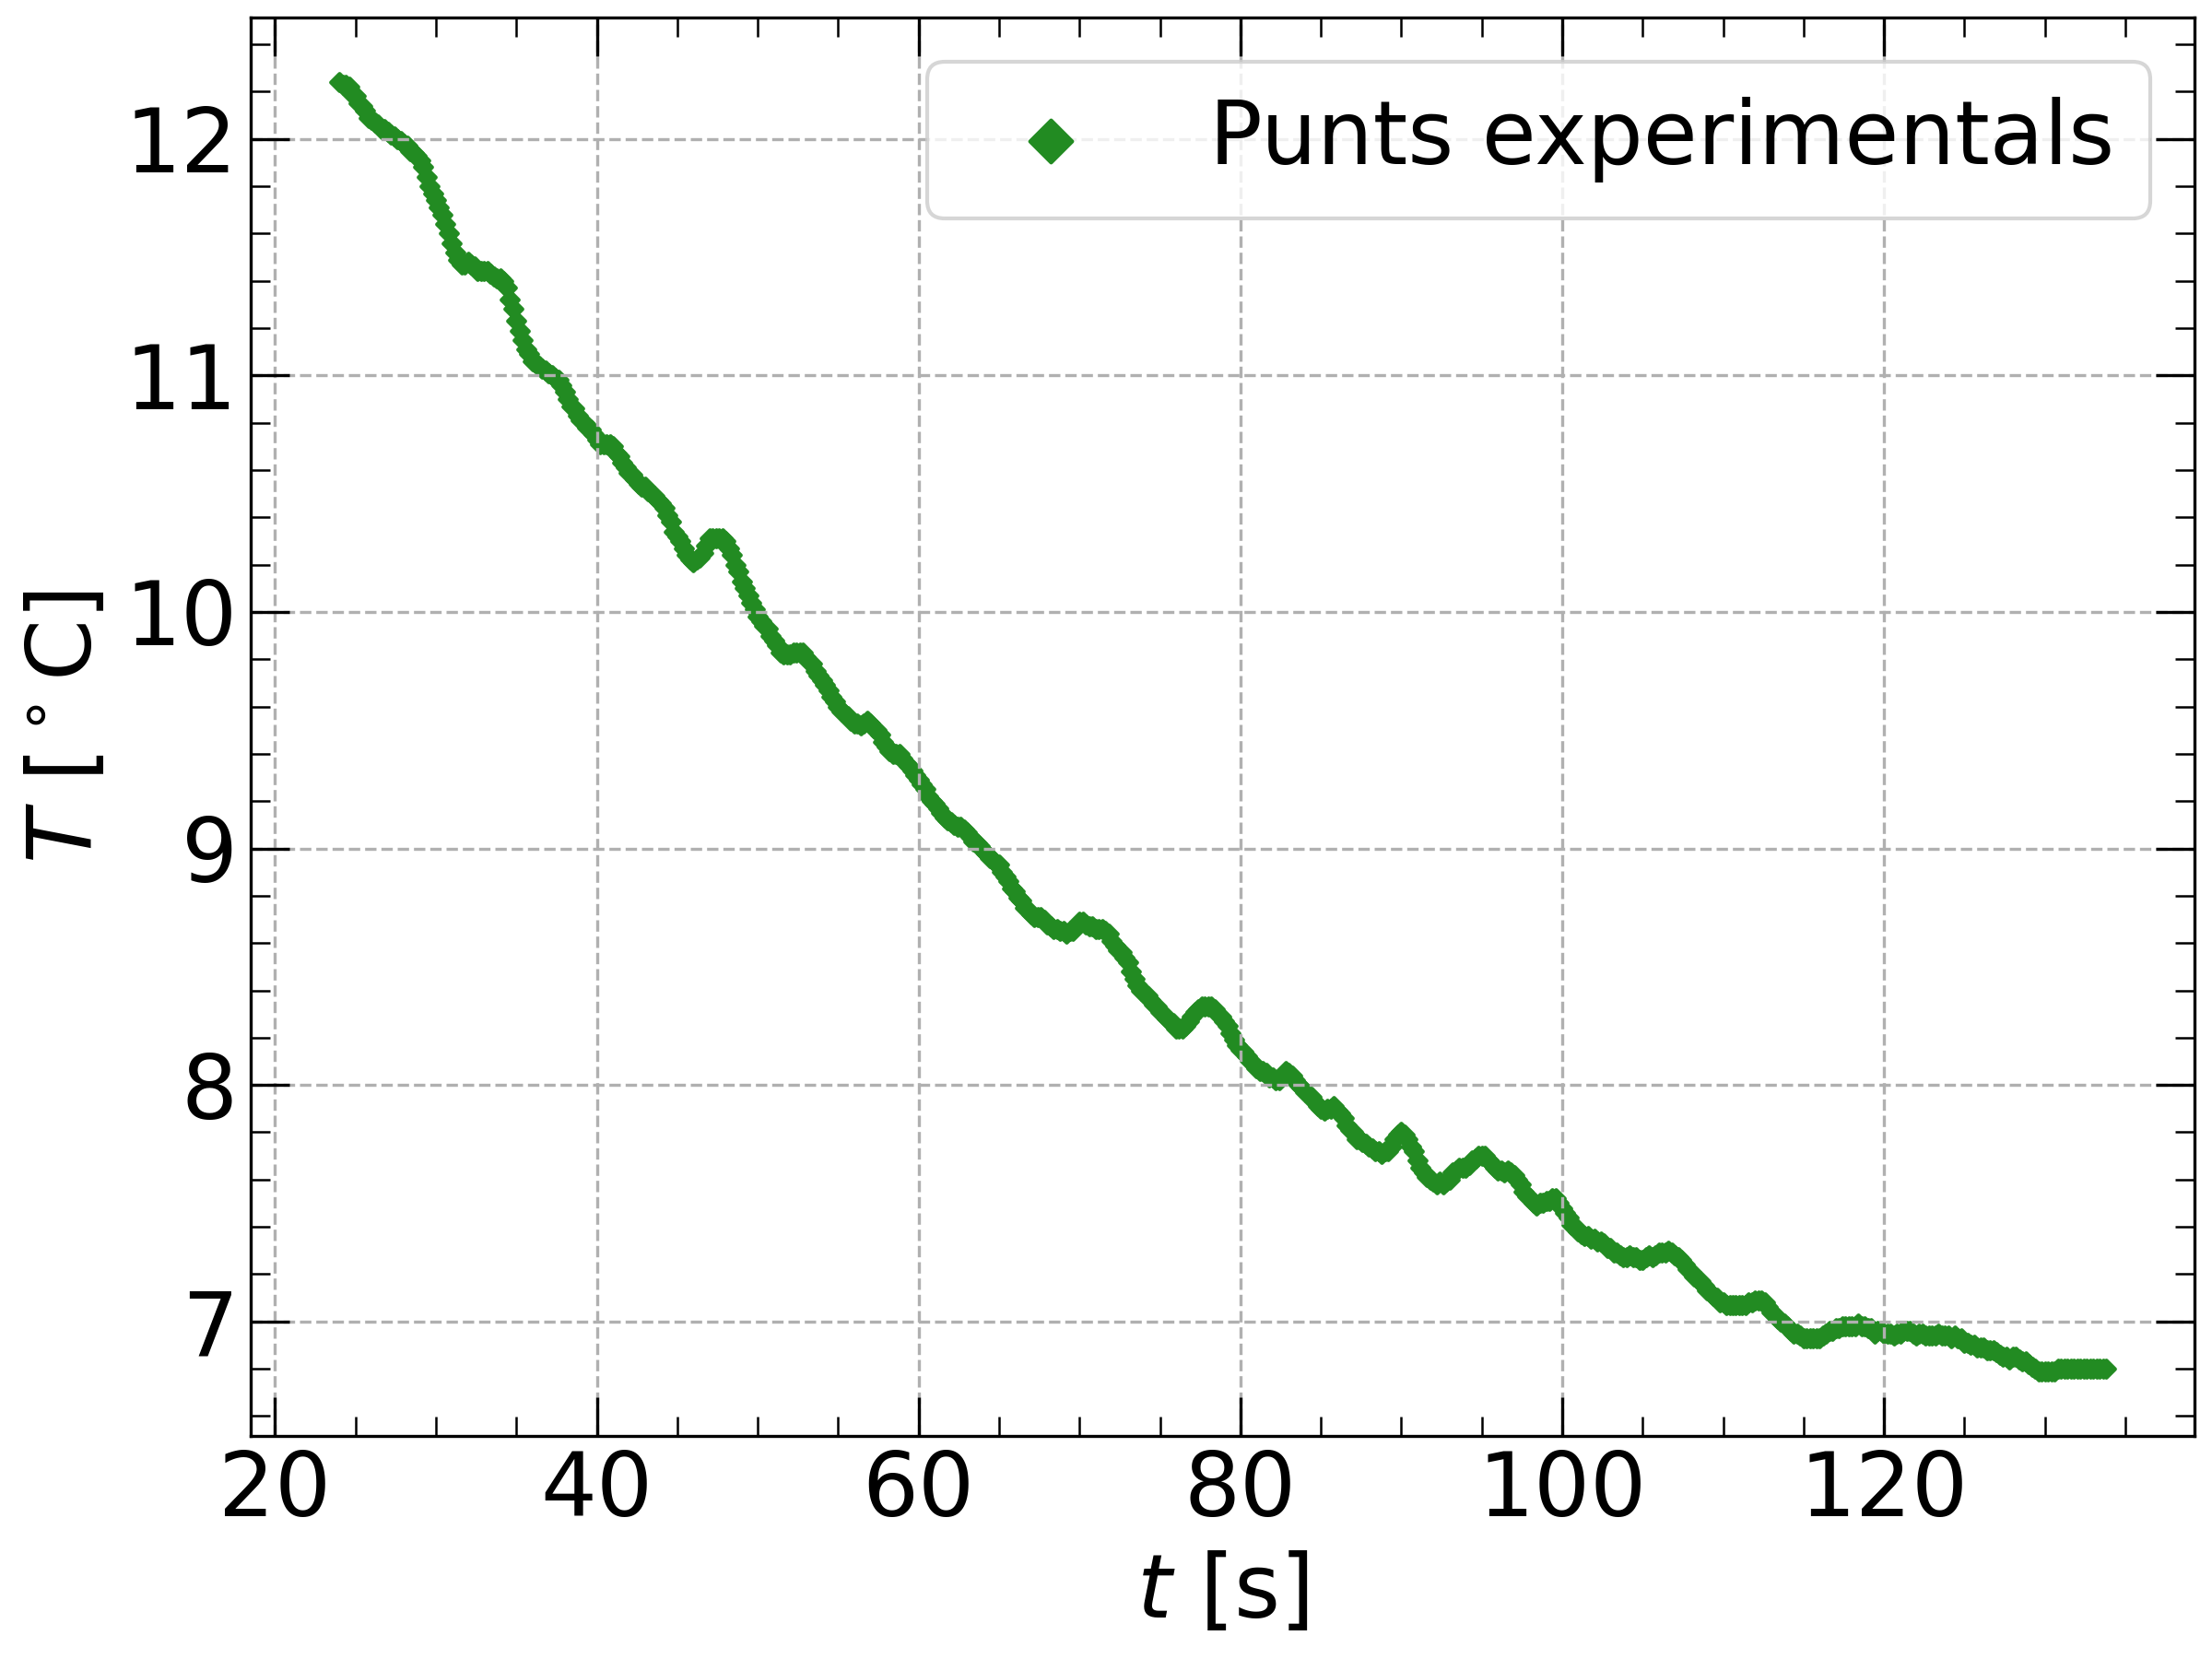
\includegraphics[width=\textwidth]{../../graphs/practica_IVc/plots/T_vs_t_tallat.png}
        \caption{} 
        \label{fig:T_vs_t_tallat}
    \end{subfigure}
    \hfill
    \begin{subfigure}[b]{0.328\textwidth}
        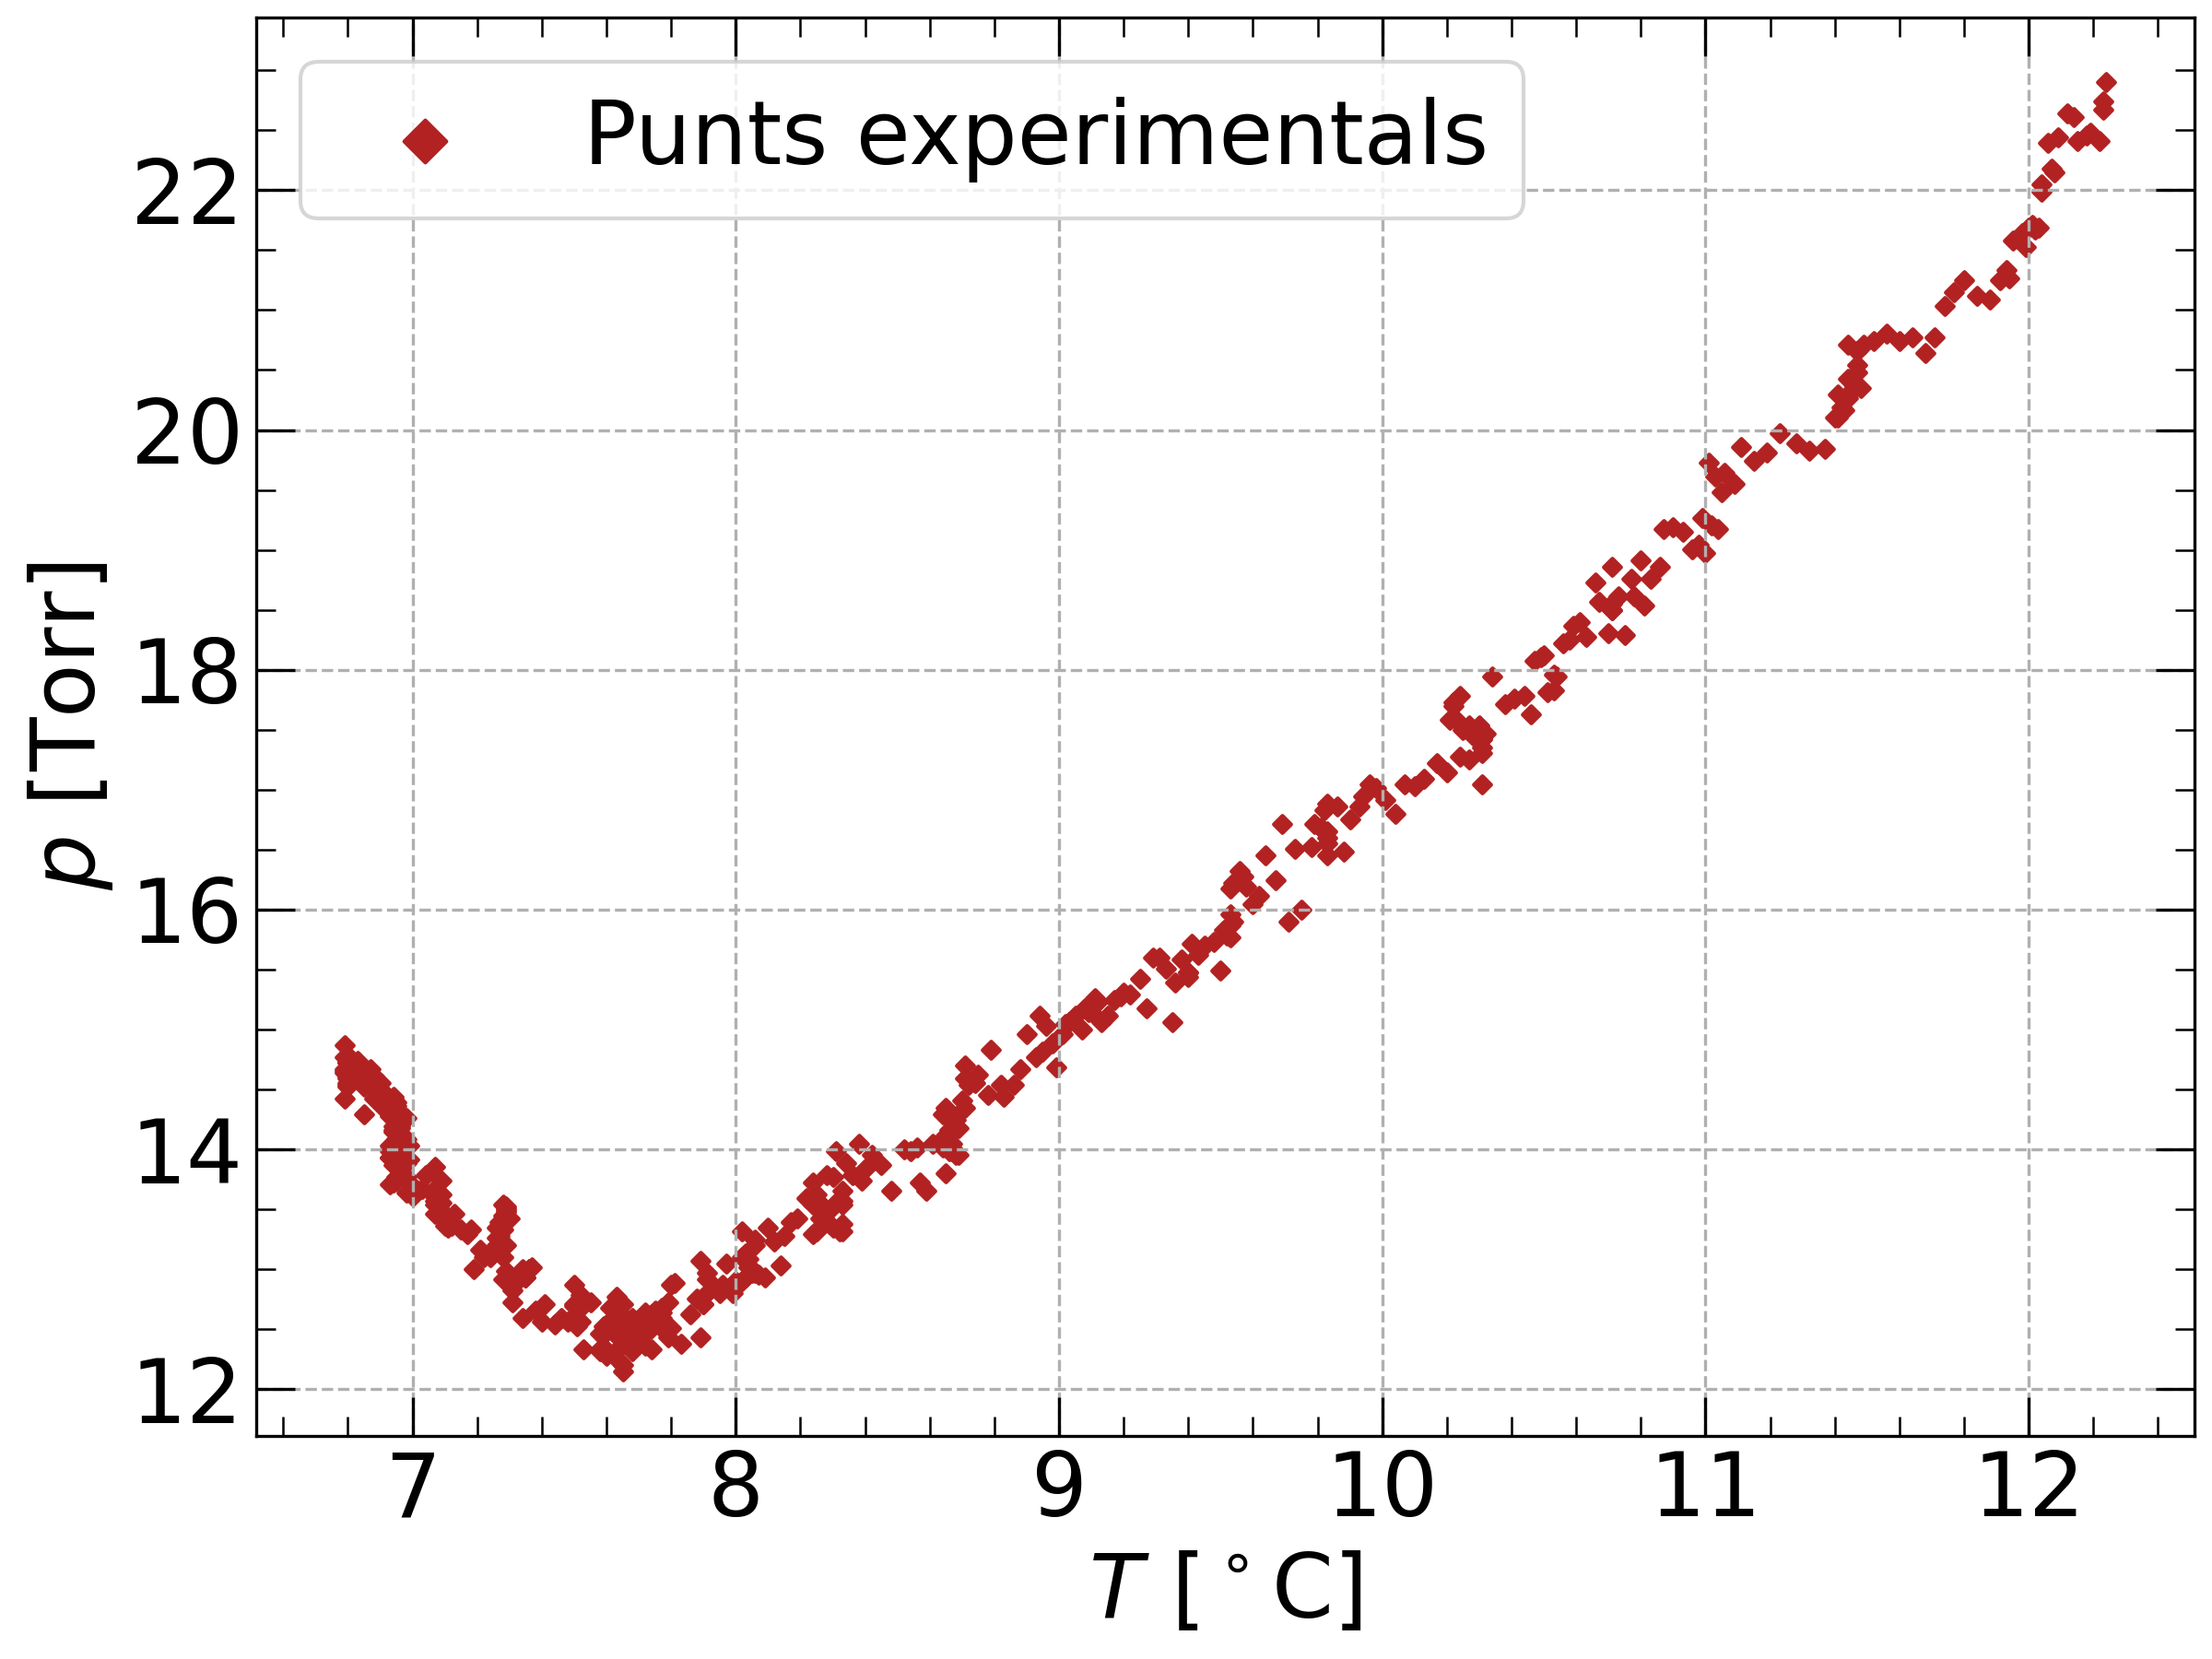
\includegraphics[width=\textwidth]{../../graphs/practica_IVc/plots/diagrama_de_fases_tallat.png}
        \caption{} 
        \label{fig:p_vs_T_tallat}
    \end{subfigure}
    \caption{(a) {\footnotesize Mesures experimentals d'evolució temporal ampliada de $p$.} (b) {\footnotesize Mesures experimentals d'evolució temporal ampliada de $T$. S'observa com la temperatura pren valors de forma oscil·lant.} (c) {\footnotesize Diagrama de fases $p$ vs $T$ ampliat del ciclohexà obtingut experimentalment. S'observa millor la corva d'quilibri i com s'arriba a un mínim de pressió. Al ser molt petites, s'ometen les incerteses a les tres repressentacions.}}
    \label{fig:tallada}
\end{figure}
\begin{multicols}{2}
S'observa a la Subfigura \ref{fig:p_vs_T_sencer} com es diferencien dos camins. El primer és un vertical, que correspon a una baixada de pressió pràcticament isotèrmica. El segon camí correspon al sistema en estat d'equilibri (comença a bullir) i el canvi de pressió comporta un canvi en la termperatura.\\\\ 
Per a poder veure aquest canvi amb més detall, es pressenta la Figura \ref{fig:tallada}, on s'omet el primer camí. Es pot observar més clarament com els canvis en la pressió i la temperatura amb el temps i, sobre tot, com evoluciona el diagrama de fases. A la Subfigura \ref{fig:fig:p_vs_T_tallat} es pot observar un mínim, que hauria de correspondre en coordenades amb el punt triple del ciclohexà.\\\\
Al llarg de l'experiència realitzada s'han pogut distingir qualitativament cada camí realitzat al diagrama de fases. Al finalitzar el primer camí s'ha observat com el fluid passa d'estar només en estat líquid a començar a bullir, només amb l'acció de baixar la pressió. Un cop ha succeït això hem pogut identificar que el sistema es trovaba al segón camí, es mantingué bullint mentre baixava bruscament la temperatura. Vam poder reconèixer el final del segón camí al obtenir el punt triple del ciclohexà. S'observa la convivència de les tres fases (sòlid, líquid i gas) en un estat d'equilibri.\\\\
Es pot observar que les dades de pressió obtingudes no s'apropen a la pressió de punt triple tabulada a la literatura que s'ha mostrat abans. Obtenim una diferència d'aproximadament\footnote{Tot i no ser una conversió idèntica ja que \(1\,\text{Torr} \simeq 0.999 999 857 533 699\, \text{mmHg}\) \cite{SI}, considerem Torr a mmHg com a unitats idèntiques en el nostre experiment.} \(32\,\text{Torr}\) entre el valor teòric i el valor experimental. Aquest error pot tenir diversos origens. Per exemple, el ciclohexà del nostre sistema pot contenir impureses que en modifiquin la pressió de punt triple, o bé les mesures realitzades amb l'ordinador tenen totes un biaix que s'ha de corretgir. Per a poder esbrinar quin és l'origen concret d'aquest error s'hauria de repetir la experiència i fer comprovacions dels nostres sistemes de buit i presa de dades amb altres substàncies, podent així realitzar les correccions pertinents.\\\\
En quant a la mesura experimental de la temperatura del punt triple observem que obtenim resultats coherents. El mínim que s'observa al diagrama de fases correspón a un valor al voltant del trobar tabulat a la literatura.\\\\
És evident que la quantitat de punts experimentals és molt alta, i que a més pressenta molt soroll provinent de les oscil·lacions de la temperatura. Podem explicar aquestes oscil·lacions si tenim en compte que el termòmetre no mesurava exclusivament la fase liquida del ciclohexà, per tant, pot haver estat afectat pels canvis de temperatura entre la fase líquida i la fase vapor. Amb l'objectiu d'aminorar aquest error experimental podem calcular una mitjana de les coordenades properes al mínim trobat experimentalment. Considerant que la distribució de punts és uniforme, fem una mitjana sense ponderar dels punts experimentals al boltant del mínim, obtenint les dades experimentals del punt triple de la Taula \ref{tau_comparativa}, on també s'afegeixen les dades tabulades per a poder comparar.
\renewcommand{\arraystretch}{1.6}
\begin{Figura}
    \centering
    \captionof{table}{\footnotesize Taula comparativa entre les dades obtingudes experimentalment (Exp.) i les tabulades a la literatura (Tab.). S'observa com les dades de la temperatura s'apropen al valor esperat de la literatura, però que el valor de la pressió difereix molt.}
    \begin{tabular}{c|c|c}
        & $p_{\text{triple}}$ [mmHg] & $T_{\text{triple}}$ [$^\circ$C] \\
        \hline\hline
        Tab. \cite{punt_triple} & 40,41 & 6,32 \\
        Exp. & $12,46\pm0,19$ & $7,63\pm0,10$
    \end{tabular}
    \label{tau_comparativa}
\end{Figura}
Notem que el valor tabulat de la temperatura de punt triple no entra dins de la incertesa obtinguda. Tot i això, el valor obtingut s'apropa. Per a obtenir una mesura més exacta s'hauria de disenyar una experiència que ens permeti no només trobar el puntr triple, sinò també poder manternir-lo en el temps i realitzar diverses mesures. També aportaria una millora fer servir un mètode de mesura de la temperatura més adient, que no es vegi perturbat per l'efecte de les bombolles del fluid al bullir.
\section{Conclusions}
En aquesta pràctica s'han realitzat diverses mesures de pressió i temperatura amb l'objectiu de, primer, observar dos sistemes diferents d'obtenció de buit i les seves limitacions, segon, fent servir el més adient trobar les coordenades de punt triple del ciclohexà.\\\\
A la primera part s'han mesurat i realitzat les correccions pertinents de la pressió obtinguda per a cada sistema de buit. S'ha pogut observar el funcionament tant de la trompa d'aigua com de la bomba d'oli rotativa a paletes i com la pressió de vapor de la substància que participa en fer el buit fixa el límit de pressió a la que pot arribar el nostre sistema. Tenint això en compte hem pogut comprovar que el sistema de buit més potent correspón al de la bomba d'oli, ja que aquest té una pressió de vapor més baixa. Tot i això, comparant amb productes que es venen al mercat, la pressió límit obtinguda amb l'oli no correspón a el límit que garanteixen els proveidors. Aquesta incoherència la podem explicar assumint que el nostre sistema de buit no treballa en condicions òptimes i poden existir, per exemple, fuites d'aire entre les juntes dels rotors de la bomba.\\\\
A la segona part hem fet servir la bomba d'oli i s'ha pogut visualitzar qualitativa i quantitativament l'obtenció de les coordenades de punt triple del coclohexà. A partir de repressentació de les nostres dades observem com es compleixen els camins teòrics al diagrama de fases. Però, la pressió de punt triple obtinguda de les nostres dades no correspón al valor que trobem a la literatura. Això pot ser originat per problemes amb el calibratge de les nostres mesures o bé per possibles impureses de la nostra mostra de ciclohexà.
\end{multicols}
\bibliographystyle{plain} 
\bibliography{referencies_IVc.bib}
\end{document}